\documentclass{article}
\usepackage[utf8]{inputenc}

\usepackage{geometry}
\usepackage{bm}
\geometry{a4paper}
\usepackage{latexsym}
%\usepackage[dvips]{graphicx}
\usepackage{epsfig}
\usepackage{amsmath}
\usepackage{amsfonts}
\usepackage{amssymb}
\usepackage{eucal}
\usepackage{mathrsfs}
\usepackage{wasysym}
\usepackage{setspace}
\usepackage{float}
\usepackage{color}
\usepackage{rotating}
\usepackage{stmaryrd}
\usepackage{lineno}

\numberwithin{equation}{section}
\frenchspacing
%%
\usepackage{amsthm}


%%%%INSERITI ADESSO%%%%
\usepackage{amsmath}
\usepackage{amsfonts}
\usepackage{amssymb}
\usepackage{amsthm}
\usepackage{mathrsfs}
\usepackage{eucal}  
\theoremstyle{definition}
\usepackage{accents}
\usepackage{array}
\usepackage{cases}
\usepackage{graphicx}
\usepackage{booktabs}
\usepackage{caption}
\usepackage{cancel}
\usepackage{bbm}
\usepackage{subfig}
\usepackage{enumitem}
\usepackage{movie15}
 \usepackage{algorithm}
\usepackage{algpseudocode}
\usepackage{tabularx}
\usepackage{longtable}
 
% Font Management
\usepackage[T1]{fontenc}       % 8 bit font encoding: includes all accents
\usepackage{bm}                % alternative to \bs provided by package amsmath
\usepackage{bbm}               % alternative to \mathbb;  usage: \mathbbm{}
%\usepackage[mathscr]{eucal}    % alternative to \mathcal; usage: \mathcal{}
\usepackage{color}             % for text in colour
\usepackage{verbatim}          % environment for commenting out blocks of text
%\usepackage{exscale}           % needed to scale cmdx fonts
%\usepackage{ae,aecompl}        % see http://www.ctan.org/tex-archive/fonts/ae
%%%%%%%%%%%%%%%%%%


\theoremstyle{plain}
\newtheorem{thm}{Theorem}[section]
\newtheorem{lem}[thm]{Lemma}
\newtheorem{prop}[thm]{Proposizione}
\newtheorem*{cor}{Corollario}

\theoremstyle{definition}
\newtheorem{defn}{Definizione}[section]
\newtheorem{conj}{Congettura}[section]
\newtheorem{exmp}{Esempio}[section]

\theoremstyle{remark}
\newtheorem*{rem}{Osservazione}
\newtheorem*{note}{Nota}

\DeclareMathOperator*{\argmin}{argmin}
\DeclareMathOperator*{\argmax}{argmax}

\newcommand{\dom}{\mathrm{dom}}
\newcommand{\im}{\mathrm{im}}
\newcommand{\sign}{\mathrm{sign}}
\newcommand{\abs}{\mathrm{abs}}
\newcommand{\e}{\mathrm{exp}}

\setlength{\textwidth}{15 cm}
\setlength{\textheight}{23.5 cm}



%%%%%%%%%%%%%%%%%%%%%%%%%%%%%%%%%%%%%%%%%%%%%%%%%%%

\usepackage[utf8]{inputenc}
\usepackage[T1]{fontenc}
\usepackage{lmodern}

\usepackage{hyperref}
\hypersetup{%
    pdfpagemode={UseOutlines},
    bookmarksopen,
    pdfstartview={FitH},
    colorlinks,
    linkcolor={blue},
    citecolor={blue},
    urlcolor={blue}
  }

%%%%%%% use PDFLATEX 

\usepackage{lipsum} %to insert random text

\usepackage{geometry} %for the margins
\newcommand\fillin[1][4cm]{\makebox[#1]{\dotfill}} %for the dotted line in the frontispiace

\usepackage{dcolumn}
\newcolumntype{d}{D{.}{.}{-1} } %to vetical align numbers in tables, along the decimal dot

\usepackage{amsmath}



%%%%%%% Local definitions
\newtheorem{osservazione}{Osservazione}% Standard LaTeX
\newtheorem{observation}{Observation}% Standard LaTeX

\newcommand{\BR}{\mathscr{B}_{\mathrm{R}}}
\newcommand{\T}[2]{T_{#2}#1}
\newcommand{\cT}[2]{T_{#2}^{*}#1}
\newcommand{\pder}[2]{\frac{\partial #1}{\partial #2}}

				 
%%%%%%%%%%%%%%%%%%%%%%%%%%%%%%%%%%%%%%%%%%%%%%%%%
%
% Inserito il codice Matlab
%
\usepackage{listings}
\usepackage{hyperref}
\usepackage{xcolor}

\definecolor{codegreen}{rgb}{0,0.6,0}
\definecolor{codegray}{rgb}{0.5,0.5,0.5}
\definecolor{codepurple}{rgb}{0.58,0,0.82}
\definecolor{backcolour}{rgb}{0.95,0.95,0.92}

\lstdefinestyle{mystyle}{
    backgroundcolor=\color{backcolour},   
    commentstyle=\color{codegreen},
    keywordstyle=\color{magenta},
    numberstyle=\tiny\color{codegray},
    stringstyle=\color{codepurple},
    basicstyle=\ttfamily\footnotesize,
    breakatwhitespace=false,         
    breaklines=true,                 
    captionpos=b,                    
    keepspaces=true,                 
    numbers=left,                    
    numbersep=4pt,                  
    showspaces=false,                
    showstringspaces=false,
    showtabs=false,                  
    tabsize=2
}

\lstset{style=mystyle}



\title{Analisi tempo-frequenza e multiscala}
\author{Giulio Nenna - 292399}
\date{Homework 1 - Riconoscimento facciale attraverso "Eigenfaces"}
\begin{document}
\maketitle
\noindent Lo scopo dell'Homework è quello di implementare e testare l'algoritmo "\textit{Eigenfaces}" per il riconoscimento facciale attraverso uno script Python. Nell'elaborato verranno presentati gli strumenti teorici a supporto dell'algoritmo, frammenti di codice salienti utilizzati e risultati computazionali ottenuti.
\\
\\
\noindent Il dataset presenta 10 ritratti facciali per ciascuno dei 40 soggetti presenti al suo interno. Vengono utilizzate immagini in scala di grigio di dimensione \(m \times n \) pixels con \(m = 112\) e \(n = 92\). Alcuni esempi di immagini utilizzate sono mostrati in Figura \ref{subject_es} 

\begin{figure}[H]
  \centering
  \subfloat[1][Soggetto 1]{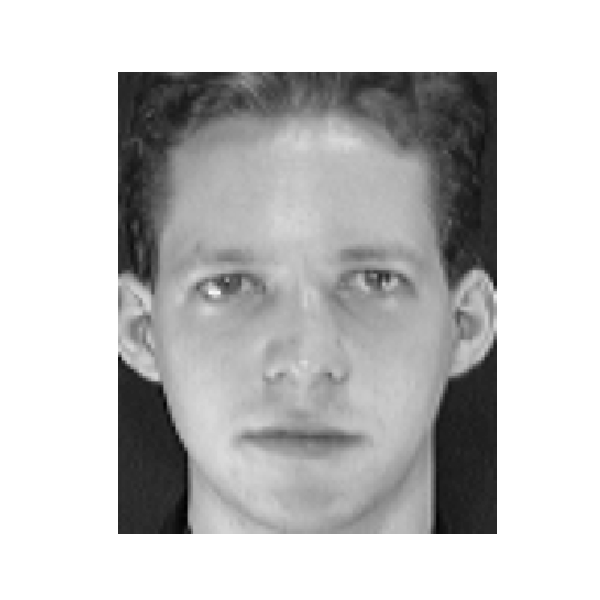
\includegraphics[scale = 0.37]{pictures/test_subject_1.pdf}}
  \subfloat[2][Soggetto 2]{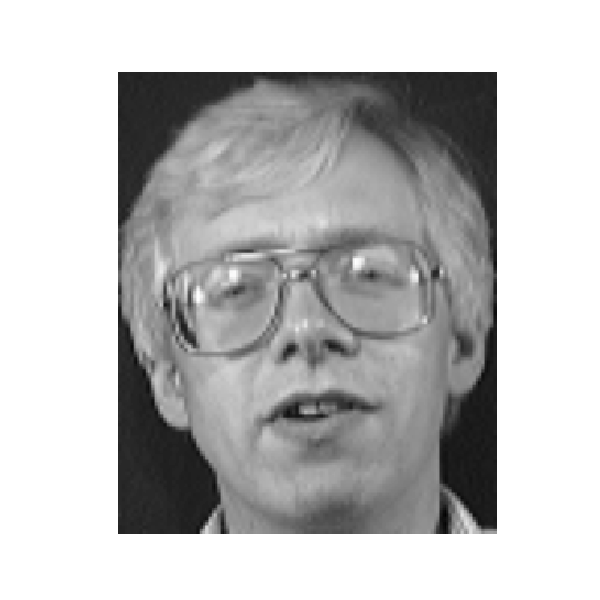
\includegraphics[scale = 0.37]{pictures/test_subject_2.pdf}}
  \subfloat[3][Soggetto 31]{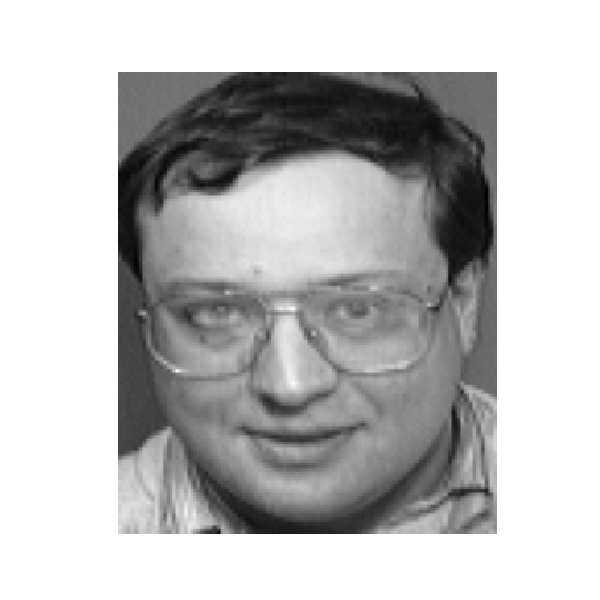
\includegraphics[scale = 0.37]{pictures/test_subject_31.pdf}}
  \caption{Alcuni esempi di immagini presenti nel dataset}
  \label{subject_es}
\end{figure}

\noindent L'algoritmo si distingue per la fase di \textbf{Training} e quella di \textbf{Testing}.
\section{Training phase}
Le immagini vengono inizialmente importate e vengono generati i dataset di \textit{Training} e \textit{testing}. In particolare nel dataset di training sono presenti le prime 6 immagini per ciascun soggetto mentre in quello di testing le restanti 4. Le immagini sono importate sotto forma di vettori \(\{f_1, f_2, \dots, f_N\}\) in \(\mathbb{R}^{mn}\). Il dataset di training contiene \(L = Np\) immagini, dove \(p\) è il rapporto tra dimensione del training set e dimensione del test set, nel nostro caso \(p = 0.6\).

\begin{lstlisting}[language=Python, caption= Data import]
faces_all = np.zeros([num_subjects*num_faces_per_subject, size])
faces_train = np.zeros([train_set_size, size])
faces_test = np.zeros([test_set_size, size])
print('Importing data...')
for i in range(num_subjects): #for each subject
    subject_faces = np.zeros([num_faces_per_subject, size]) #array containing all faces of the subject
    for j in range(num_faces_per_subject): #for each face
        f=path+'/s'+str(i+1)+'/'+str(j+1)+'.pgm' #compose filepath
        img = pgm.read_pgm(f) #read the file (2D array of shape m by n)
        img = img.reshape(size) #reshape the img into a 1D array
        subject_faces[j,:] = img 
    
    faces_all[i*num_faces_per_subject:(i+1)*num_faces_per_subject,:] = subject_faces
    faces_train[i*int(num_faces_per_subject*train_test_ratio):(i+1)*int(num_faces_per_subject*train_test_ratio),:] = \
        subject_faces[0:int(num_faces_per_subject*train_test_ratio),:]
    faces_test[i*int(num_faces_per_subject*(1-train_test_ratio)):(i+1)*int(num_faces_per_subject*(1-train_test_ratio)),:] = \
            subject_faces[int(num_faces_per_subject*train_test_ratio):num_faces_per_subject,:]
\end{lstlisting}

\noindent Viene adesso calcolata la faccia media \(\tilde{f} = \frac{1}{L}  \sum \limits_{l=1}^{L} f_l\) e il dataset di training viene centrato rispetto alla faccia media, ottenendo nuovi vettori \(\phi_l = f_l - \tilde{f}\) con \(l \in \{1, \dots, L\}\).

\begin{lstlisting}[language=Python, caption= Centering data]
L =  faces_train.shape[0]
mean_face = faces_train.mean(axis = 0) #compute mean face
faces_train_center = faces_train-mean_face #centering the dataset (is the matrix Phi^T)
\end{lstlisting}

 \noindent A questo punto l'idea è quella di trovare una particolare base ortonormale \(\{u_1, \dots,u_{K}\}\) con \(u_i \in \mathbb{R}^{mn}, i=1,\dots K\) tale per cui:
\begin{eqnarray*}
    \phi_l = \tilde{f} +  \sum \limits_{n\geq 1} \alpha_n u_n \\
|\alpha_1| \geq |\alpha_2| \geq, ..., \geq |\alpha_{K}|
\end{eqnarray*}
La seconda condizione afferma che la base ortonormale che si sta cercando è tale per cui le componenti sono ordinate per "importanza". Questo concetto è fondamentale per la pratica della riduzione dimensionale: se si riesce a trovare una base di rappresentazione delle immagini per cui le prime componenti sono più importanti delle ultime, allora sarà possibile rappresentare le immagini utilizzando il sottoinsieme delle prime componenti perdendo la minor quantità di informazioni possibile.
\\
\\
Sia \(\lambda_1\) il coefficiente rispetto alla prima componente della base \(u_1\) per la generica immagine \(\phi_l\). 
\[
    \lambda_1 = \left\langle\phi_l, u_1 \right\rangle  
    \]
Sia \(\Phi^T\) la matrice contenente per ciascuna riga le immagini di training:
\[\Phi^T = \begin{bmatrix}
    \phi_1^T \\
    \phi_2^T \\
    \vdots \\
    \phi_L^T
\end{bmatrix}
    \]
\\
Allora il problema della ricerca della prima componente della base \(u_1\) che massimizza in media il modulo del relativo coefficiente per ogni immagine di training si formalizza come:
\begin{equation}
    \max_{\| x \| = 1 } \frac{1}{L}  \sum \limits_{l=1}^{L} | \langle \phi_l, x\rangle|^2 = \max_{\| x \| = 1 } \frac{1}{L} \| \Phi^T x \| ^2_2 = \max_{\| x \| = 1 } \left\langle \frac{1}{L}\Phi \Phi^T x, x \right\rangle = \lambda_1.
\end{equation}
In particolare \(\frac{1}{L}\Phi \Phi^T\) è la matrice di varianza-covarianza campionaria di \(\{\phi_1, ... \phi_L\}\) e \(\lambda_1\) è il suo più grande autovalore in modulo. \(u_1\) sarà pertanto l'autovettore relativo a \(\lambda_1\).
Per la ricerca della seconda componente il procedimento è lo stesso, imponendo l'ortogonalità rispetto alla prima componente:
\[
    \max_{\|x\| = 1, \, x \bot u_1 } \left\langle \frac{1}{L}\Phi \Phi^T x, x \right\rangle = \lambda_2.
\]
La ricerca della particolare base che stiamo cercando si riduce pertanto al problema del calcolo di autovalori e autovettori della matrice  \(\frac{1}{L}\Phi \Phi^T\).
\\
\\
Un'importante dettaglio implementativo è dato dalla dimensione della matrice \(\Phi\Phi^T \in \mathbb{R}^{mn \times mn}\). La quantità \(mn\)  è potenzialmente molto grande (nel nostro caso \(mn \sim 10^3\)), rendendo il calcolo degli autovalori e autovettori un'operazione computazionalmente molto onerosa. Questo problema può tuttavia essere aggirato se si considera che \(\text{Rank}(\Phi\Phi^T) \leq L \) e che gli autovalori della matrice \(\Phi^T \Phi\) sono gli stessi della matrice \(\Phi \Phi^T\). Inoltre:
\[ \Phi\Phi^T x = \lambda x \iff \Phi^T \Phi \Phi^T x = \lambda \Phi^T x
    \]
Pertanto se \(y = \Phi^T x\) è un autovettore di \(\Phi^T \Phi\), allora \(x = \Phi y\) sarà il corrispondente autovettore di \( \Phi\Phi^T \). Il calcolo degli autovettori può pertanto essere eseguito sulla matrice \(\Phi^T \Phi \in \mathbb{R}^{L \times L}\) con \(L \ll mn \) alleggerendo di molto i costi computazionali.
\\
\\
La particolare base che stiamo cercando sarà quindi data da  \(V = \{v_1, \dots, v_L\}\) dove 
\[ v_i = \Phi u_i \quad i = \{1, \dots, L\},\]
\[u_i \text{ autovettore di } \Phi^T\Phi \text{ relativo all'autovalore } \lambda_i ,\]
\[\lambda_1 \geq \lambda_2 \geq \dots \geq \lambda_L.\]
Una volta ottenuta la base \(V\) è possibile scegliere le sue prime \(L'<L\) componenti ottenendo una base \(V' = \{v_1, \dots , v_{L'}\}\) che approssima \(V\). È possibile quantificare la perdita di informazioni se si utilizza la base \(V'\) piuttosto che \(V\) per rappresentare le immagini. In particolare possiamo decidere il numero di componenti trattenute \(L'\) calcolando la varianza trattenuta dalla base:
\[\frac{ \sum \limits_{l=1}^{L'} \lambda_l}{ \sum \limits_{l=1}^{L}\lambda_l } > \alpha\]
dove \(\alpha \in [0,1]\) è una soglia decisa a priori. Al crescere di \(\alpha\) crescerà il numero di componenti necessarie a trattenere la varianza desiderata.
Quanto spiegato fin ora può essere eseguito attraverso i seguenti comandi:

\begin{lstlisting}[language=Python]
#computing modified covariance matrix (Phi^T * Phi)
cov_mat_mod = 1/L * (faces_train_center @ faces_train_center.transpose()) 
#computing eigenvalues and eigenvectors
eig_val, eig_vec = np.linalg.eig(cov_mat_mod)
#sorting eigenvalues and eigenvectors in decreasing  order
sort_mask = np.argsort(eig_val)[::-1]
eig_val = eig_val[sort_mask]
eig_vec = eig_vec[:, sort_mask]
#computing the cumulative explained variance
explained_variance_cum = (eig_val/eig_val.sum()).cumsum() 

threshold_mask = explained_variance_cum<variance_threshold
num_pcs_kept = (threshold_mask).sum()
#computing eigenvalues of the original covariance matrix
eigenfaces = faces_train_center.transpose() @ eig_vec[:,threshold_mask] 
#normalize by columns the eigenvectors (eigenfaces is now an orthonormal matrix)
eigenfaces = normalize(eigenfaces, axis=0, norm='l2') # is the matrix V'
#project train faces onto the eigenfaces space
faces_train_projected = faces_train_center @ eigenfaces
\end{lstlisting}

\noindent Un dettaglio da non sottovalutare è dato dal fatto che la matrice \(V = [v_1, v_2, \dots v_L]\) è stata ottenuta dal calcolo degli autovettori \(\{u_1, u_2, \dots u_L\}\) ciascuno moltiplicato per \(\Phi\). Se \(\{u_1, u_2, \dots u_L\}\) è un insieme di vettori a norma 1, l'insieme \(\{v_1, v_2,\dots v_L \}\) non lo è, pertanto la matrice \(V\) va normalizzata per colonne.
\\
\\
Una volta calcolata la matrice \(V'\) relativa alla base \(V'\) è possibile proiettare le facce dallo spazio originale a \(V'\):
\[
\phi_l' = V'^T\phi_l \quad l = 1 \dots L
\]
In notazione matriciale:
\[
    \Phi'^T = \begin{bmatrix}
        \phi_1'^T \\
        \phi_2'^T \\
        \vdots \\
        \phi_L'^T
    \end{bmatrix} \quad \Phi'^T = \Phi^T V'  \quad \Phi'^T \in \mathbb{R}^{L \times L'} 
\]
\begin{lstlisting}[language=Python]
#project train faces onto the eigenfaces space
faces_train_projected = faces_train_center @ eigenfaces # Phi'^T = Phi^T * V'
\end{lstlisting}

%\bibliographystyle{plain} % We choose the "plain" reference style
%\bibliography{refs} % Entries are in the refs.bib file


\end{document}